\subsection{Massive Static Yukawa Results}
\label{sec:static_yukawa}

The next simplest model that we consider is a non-relativistic approximation to the Yukawa model, which is commonly referred to as the massive static Yukawa model \cite{PhysRevD.103.014021}.
This model is taken as the limit of the full Yukawa model of infinitely heavy fermions, and bosons at rest relative to the fermions that emit/absorb them.

The second-quantized Hamiltonian for this model is given by:
\begin{equation}
    \label{eq:static-yukawa}
    H = C_f b^\dagger b + C_b a^\dagger a + g b^\dagger b \left( a + a^\dagger \right)
\end{equation}
where there is only one fermionic mode and one bosonic mode. 

\begin{figure*}
    \label{fig:static_yukawa}
    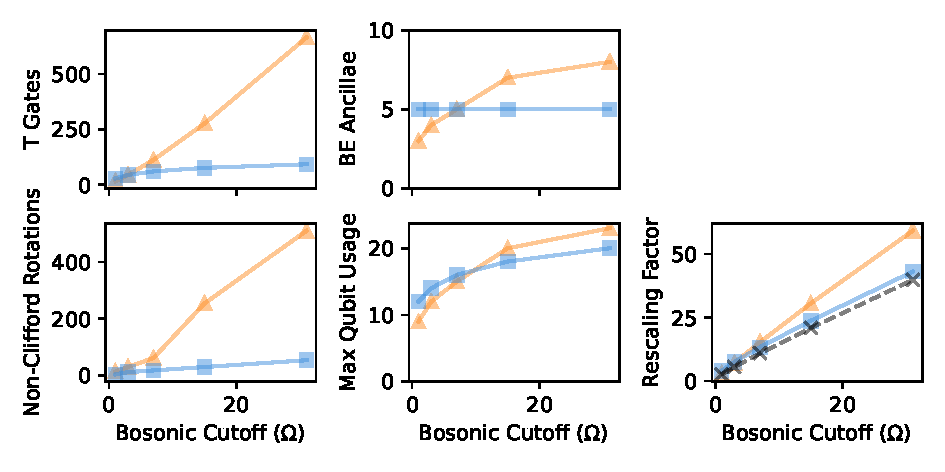
\includegraphics[width = 16cm]{figures/static_yukawa.pdf}
    \caption{
        \textbf{Static Massive Yukawa}
        The number of T gates (upper-left), number of non-Clifford rotations (lower-left), block-encoding ancillae (upper-middle), maximum number of qubits used (lower-middle), and rescaling factor (lower-right) are shown as a function of the bosonic occupation cutoff ($\Omega$).
        The parameters $C_f$, $C_b$, and $g$ are set to $1$ for all data points.
        Results for the Pauli Expansion method are shown as the orange triangles and results for LOBE are shown as the blue circles.
        The optimal rescaling factor, which is given by the L2 norm of the Hamiltonian, is shown as the dashed black crosses.
    }
\end{figure*}

As this model is restricted to one fermionic and one bosonic mode, we compare the spacetime costs of the different block-encoding methods as a function of the bosonic occupation cutoff ($\Omega$).
Similar to the quartic harmonic oscillator, the Pauli Expansion method results in lower spacetime costs when the bosonic cutoff is low.
However, the LOBE constructions have better asymptotic scaling with resect to $\Omega$ and crossover points exist for all metrics, above which LOBE results in lower cost constructions.
For the time-complexity, this crossover point occurs at $\Omega = 3$ for the number of T gates and the LOBE constructions require fewer non-Clifford rotations at all values of $\Omega$.
For the space-complexity, this crossover point occurs at $\Omega = 7$ for the number of block-encoding ancillae and $\Omega = 15$ for the maximum number of qubits.
Finally, for the rescaling factor, this crossover point occurs at $\Omega = 15$.